\section{问题一：盘入运动状态模型的建立与求解}
\subsection{问题一的建模思路}
问题一要求给出0--300 s内龙头、龙身和龙尾各把手的位置与速度。由于所有把手均约束在同一条盘入螺线上，而相邻板凳之间又由固定把手间距连接，因此可将问题拆为两个层次：先确定龙头前把手的螺线参数，再沿同一条曲线递推其余把手的参数。

本文采用极坐标描述螺线。原因在于，题目给出的轨迹本质上是等距螺线，其核心几何量是“半径随极角线性变化”；这一关系在极坐标下直接写成代数式，而在直角坐标中则会引入额外的旋转与曲率表达。故位置求解的关键量由二维坐标降为单一参数$\theta$。

\subsection{等距螺线方程的建立}
设螺线中心为原点$O$，$x$轴水平向右，$y$轴竖直向上。根据题图约定，点A位于正$x$轴上，龙头沿顺时针方向向内盘入。等距螺线满足
\[
r(\theta+2\pi)-r(\theta)=p.
\]
若取半径关于极角线性变化，则有
\[
r(\theta)=b\theta,\qquad b=\frac{p}{2\pi}.
\]
问题一中$p=0.55$ m，所以
\[
b=\frac{0.55}{2\pi}.
\]
将极坐标转为直角坐标，得到把手中心的位置表达式
\[
\begin{cases}
x(\theta)=r(\theta)\cos\theta,\\
y(\theta)=r(\theta)\sin\theta.
\end{cases}
\]
因此，一旦确定某一把手对应的螺线参数$\theta$，其平面位置就被唯一确定。

为直观说明上述极坐标建模过程，等距螺线的几何要素示意图如下。

\begin{figure}[H]
\centering
\placeholderimage{5.4cm}{
图位预留：等距螺线极坐标建模示意图。\\[0.4em]
图中标出极点$O$、极角$\theta$、半径$r$、螺距$p$，\\
并标明$r=b\theta$与相邻两圈半径差$p$之间的关系。
}
\caption{等距螺线极坐标建模示意}
\label{fig:q1-spiral-model}
\end{figure}

\subsection{龙头前把手的弧长关系}
题目给定龙头前把手的速度为1 m/s。对于参数曲线
\[
x(\theta)=b\theta\cos\theta,\qquad y(\theta)=b\theta\sin\theta,
\]
其导数为
\[
\frac{dx}{d\theta}=b\cos\theta-b\theta\sin\theta,\qquad
\frac{dy}{d\theta}=b\sin\theta+b\theta\cos\theta.
\]
故弧长微元满足
\[
ds=\sqrt{\left(\frac{dx}{d\theta}\right)^2+\left(\frac{dy}{d\theta}\right)^2}\,d\theta
=b\sqrt{1+\theta^2}\,d\theta.
\]
于是从0到$\theta$的弧长函数为
\[
S(\theta)=\int_0^\theta b\sqrt{1+u^2}\,du
=\frac{b}{2}\Bigl[\theta\sqrt{\theta^2+1}+\operatorname{asinh}(\theta)\Bigr].
\]
该函数把螺线参数与沿曲线行进距离联系起来，因此龙头位置可由弧长反解得到。

\subsection{初始角$\theta_0$的确定}
题目说明龙头从第16圈处开始盘入。等距螺线绕原点一圈对应极角变化$2\pi$，第16圈对应
\[
\theta_0=16\times2\pi=32\pi.
\]
在本文的坐标约定下，$\theta_0=32\pi$对应正$x$轴方向，与题图中A点位于正$x$轴一致。由于龙头顺时针向内运动，半径随时间减小，等价于$\theta$随时间减小。

设龙头前把手在时刻$t$的参数为$\theta_H(t)$，则
\[
S(\theta_0)-S\!\left(\theta_H(t)\right)=v_H t,\qquad v_H=1.
\]
即
\[
S\!\left(\theta_H(t)\right)=S(\theta_0)-v_H t.
\]
由此得到一元单调方程。求得$\theta_H(t)$后，再代入坐标转换式即可恢复龙头前把手的位置。

\subsection{相邻把手递推模型}
龙头前把手确定后，其余把手必须满足相邻把手中心距离固定。龙头板的前后把手中心距为
\[
\ell_H=3.41-2\times0.275=2.86\ \text{m},
\]
普通龙身板和龙尾板的前后把手中心距为
\[
\ell_B=2.20-2\times0.275=1.65\ \text{m}.
\]

相邻把手、板凳实体与中心线之间的几何关系示意图如下，该图用于说明后续递推约束与碰撞矩形模型的共同几何来源。

\begin{figure}[H]
\centering
\placeholderimage{5.0cm}{
图位预留：相邻把手与板凳实体几何关系图。\\[0.4em]
图中标出前后把手中心、把手间距$\ell_H,\ell_B$、板长、板宽$w$、\\
把手孔到板端的外延，以及由把手连线确定的板凳中心轴。
}
\caption{相邻把手与板凳实体的几何关系示意}
\label{fig:q1-bench-geometry}
\end{figure}

记第$i$个把手在时刻$t$对应的螺线参数为$\theta_i(t)$，位置为
\[
P_i(t)=\bigl(x(\theta_i(t)),y(\theta_i(t))\bigr).
\]
已知$P_i(t)$后，第$i+1$个把手仍位于同一条螺线上，且满足
\[
\left\|P_{i+1}(t)-P_i(t)\right\|_2=d_i,
\qquad
d_i=
\begin{cases}
\ell_H, & i=0,\\
\ell_B, & i=1,2,\ldots,222.
\end{cases}
\]
展开得
\[
\left[x(\theta_{i+1})-x(\theta_i)\right]^2+
\left[y(\theta_{i+1})-y(\theta_i)\right]^2=d_i^2.
\]
由于板凳龙由头至尾单向排布，后一把手在螺线上对应更外侧的参数值，即$\theta_{i+1}>\theta_i$。在该单调区间内求解上式，可排除非物理解。于是，问题一的几何状态由“路径约束+间距约束”唯一确定。

\subsection{速度计算}
对后续把手，速度按相邻时刻的轨迹长度差分得到。若记第$i$个把手在相邻时刻的位置为$P_i(t-\Delta t)$和$P_i(t+\Delta t)$，则可用中心差分近似
\[
v_i(t)\approx
\frac{\left\|P_i(t+\Delta t)-P_i(t-\Delta t)\right\|_2}{2\Delta t}.
\]
端点时刻使用单侧差分。该做法与逐秒输出要求一致，也避免了显式求解隐函数导数。

\subsection{求解流程}
\begin{algorithm}[H]
\caption{问题一逐时刻位置与速度求解流程}
\label{alg:q1-state}
\textbf{Input:} 螺距$p=0.55$，整数时刻$t=0,1,\ldots,300$，把手间距$d_i$。\\
\textbf{Output:} 全部把手的位置表与速度表。
\begin{enumerate}[label=\arabic*:, leftmargin=2.6em, itemsep=0.2em]
\item 令$b=p/(2\pi)$，建立等距螺线$r(\theta)=b\theta$。
\item 对每个时刻$t$，求解弧长方程$S(\theta_0)-S(\theta_H(t))=v_Ht$，得到龙头前把手参数$\theta_H(t)$。
\item 对$i=1,\ldots,223$，在$\theta_i>\theta_{i-1}$分支上求解$\|P_i(t)-P_{i-1}(t)\|_2=d_i$。
\item 将所有$\theta_i(t)$代入坐标变换，得到$(x_i(t),y_i(t))$。
\item 对离散位置序列作差分，得到各把手速度$v_i(t)$。
\item \textbf{return} 位置表与速度表。
\end{enumerate}
\end{algorithm}
上述流程把“轨迹反解”和“链式递推”分离开来，便于逐时刻稳定求解。

根据该流程得到的板凳龙在盘入螺线上的某一时刻整体排布示意图如下。

\begin{figure}[H]
\centering
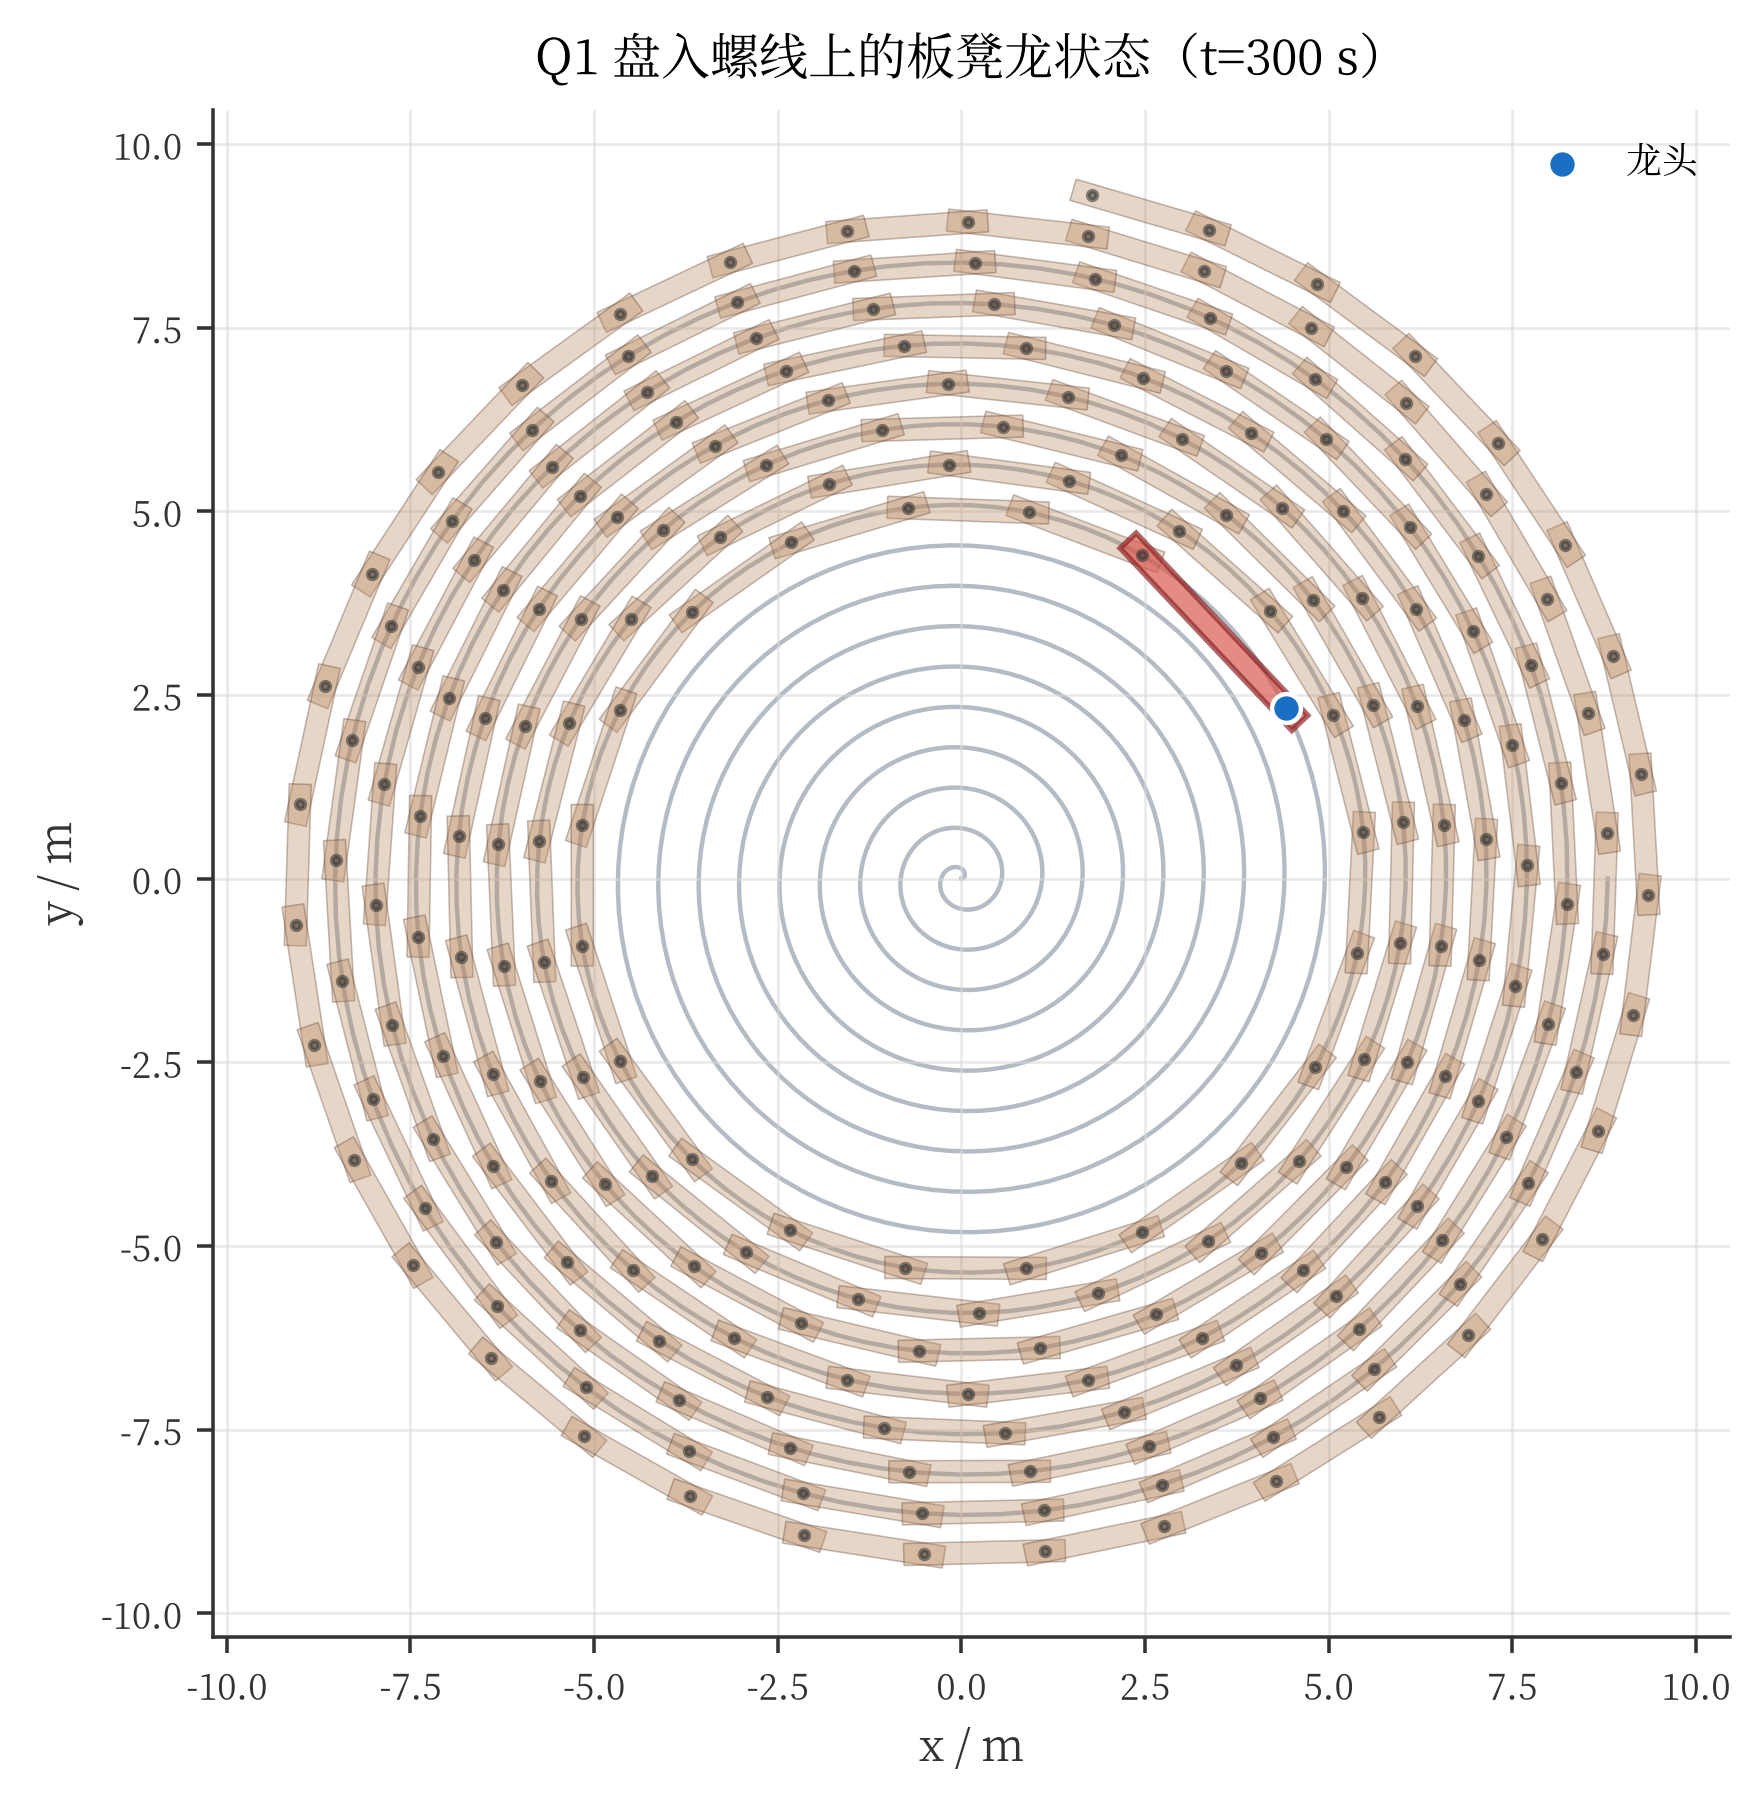
\includegraphics[width=0.92\textwidth]{figures/python/q1_spiral_bench_snapshot.png}
\caption{板凳龙在盘入螺线上的运动状态截取}
\label{fig:q1-spiral-snapshot}
\end{figure}

\subsection{结果分析}
按上述模型输出的0--300 s数据中，位置表规模为449行、302列，速度表规模为225行、302列，覆盖全部224个把手和301个整数时刻。相邻把手距离的最大误差为
\[
8.32\times10^{-12}\ \text{m},
\]
平均绝对误差为
\[
4.64\times10^{-14}\ \text{m}.
\]
这说明逐节递推在数值上很好地保持了板凳连接约束。与稠密折线基线在0 s、60 s、120 s、180 s、240 s和300 s处比较，最大坐标差为$0.0153$ m，说明模型输出与离散路径近似结果保持一致。

\begin{table}[H]
\centering
\caption{问题一位置抽样表}
\label{tab:q1-position}
\begingroup
\small
\setlength{\tabcolsep}{2pt}
\begin{tabularx}{\textwidth}{lCCCCCC}
\toprule
项目 & 0 s & 60 s & 120 s & 180 s & 240 s & 300 s\\
\midrule
龙头 $x$ (m) & 8.800000 & 5.799209 & -4.084887 & -2.963609 & 2.594494 & 4.420274\\
龙头 $y$ (m) & 0.000000 & -5.771092 & -6.304479 & 6.094780 & -5.356743 & 2.320429\\
第1节龙身 $x$ (m) & 8.363824 & 7.456758 & -1.445473 & -5.237118 & 4.821221 & 2.459489\\
第1节龙身 $y$ (m) & 2.826544 & -3.440399 & -7.405883 & 4.359627 & -3.561949 & 4.402476\\
第51节龙身 $x$ (m) & -9.518732 & -8.686317 & -5.543150 & 2.890455 & 5.980011 & -6.301346\\
第51节龙身 $y$ (m) & 1.341137 & 2.540108 & 6.377946 & 7.249289 & -3.827758 & 0.465829\\
第101节龙身 $x$ (m) & 2.913983 & 5.687116 & 5.361939 & 1.898794 & -4.917371 & -6.237722\\
第101节龙身 $y$ (m) & -9.918311 & -8.001384 & -7.557638 & -8.471614 & -6.379874 & 3.936008\\
第151节龙身 $x$ (m) & 10.861726 & 6.682311 & 2.388757 & 1.005154 & 2.965378 & 7.040740\\
第151节龙身 $y$ (m) & 1.828753 & 8.134544 & 9.727411 & 9.424751 & 8.399721 & 4.393013\\
第201节龙身 $x$ (m) & 4.555102 & -6.619664 & -10.627211 & -9.287720 & -7.457151 & -7.458662\\
第201节龙身 $y$ (m) & 10.725118 & 9.025570 & 1.359847 & -4.246673 & -6.180726 & -5.263384\\
龙尾（后） $x$ (m) & -5.305444 & 7.364557 & 10.974348 & 7.383896 & 3.241051 & 1.785033\\
龙尾（后） $y$ (m) & -10.676584 & -8.797992 & 0.843473 & 7.492370 & 9.469336 & 9.301164\\
\bottomrule
\end{tabularx}
\endgroup
\end{table}

\begin{table}[H]
\centering
\caption{问题一速度抽样表}
\label{tab:q1-speed}
\begingroup
\small
\setlength{\tabcolsep}{2pt}
\begin{tabularx}{\textwidth}{lCCCCCC}
\toprule
项目 & 0 s & 60 s & 120 s & 180 s & 240 s & 300 s\\
\midrule
龙头 (m/s) & 1.000000 & 1.000000 & 1.000000 & 1.000000 & 1.000000 & 1.000000\\
第1节龙身 (m/s) & 0.999971 & 0.999961 & 0.999945 & 0.999917 & 0.999859 & 0.999709\\
第51节龙身 (m/s) & 0.999742 & 0.999662 & 0.999538 & 0.999331 & 0.998941 & 0.998065\\
第101节龙身 (m/s) & 0.999575 & 0.999453 & 0.999269 & 0.998971 & 0.998435 & 0.997302\\
第151节龙身 (m/s) & 0.999448 & 0.999299 & 0.999078 & 0.998727 & 0.998115 & 0.996861\\
第201节龙身 (m/s) & 0.999348 & 0.999180 & 0.998935 & 0.998551 & 0.997894 & 0.996574\\
龙尾（后） (m/s) & 0.999311 & 0.999136 & 0.998883 & 0.998489 & 0.997816 & 0.996478\\
\bottomrule
\end{tabularx}
\endgroup
\end{table}

由表\ref{tab:q1-speed}可见，龙头速度保持为1 m/s，其余关键把手速度随时间略有下降。为更直观比较不同位置把手的速度变化，关键把手速度随时间变化曲线如下。

\begin{figure}[H]
\centering
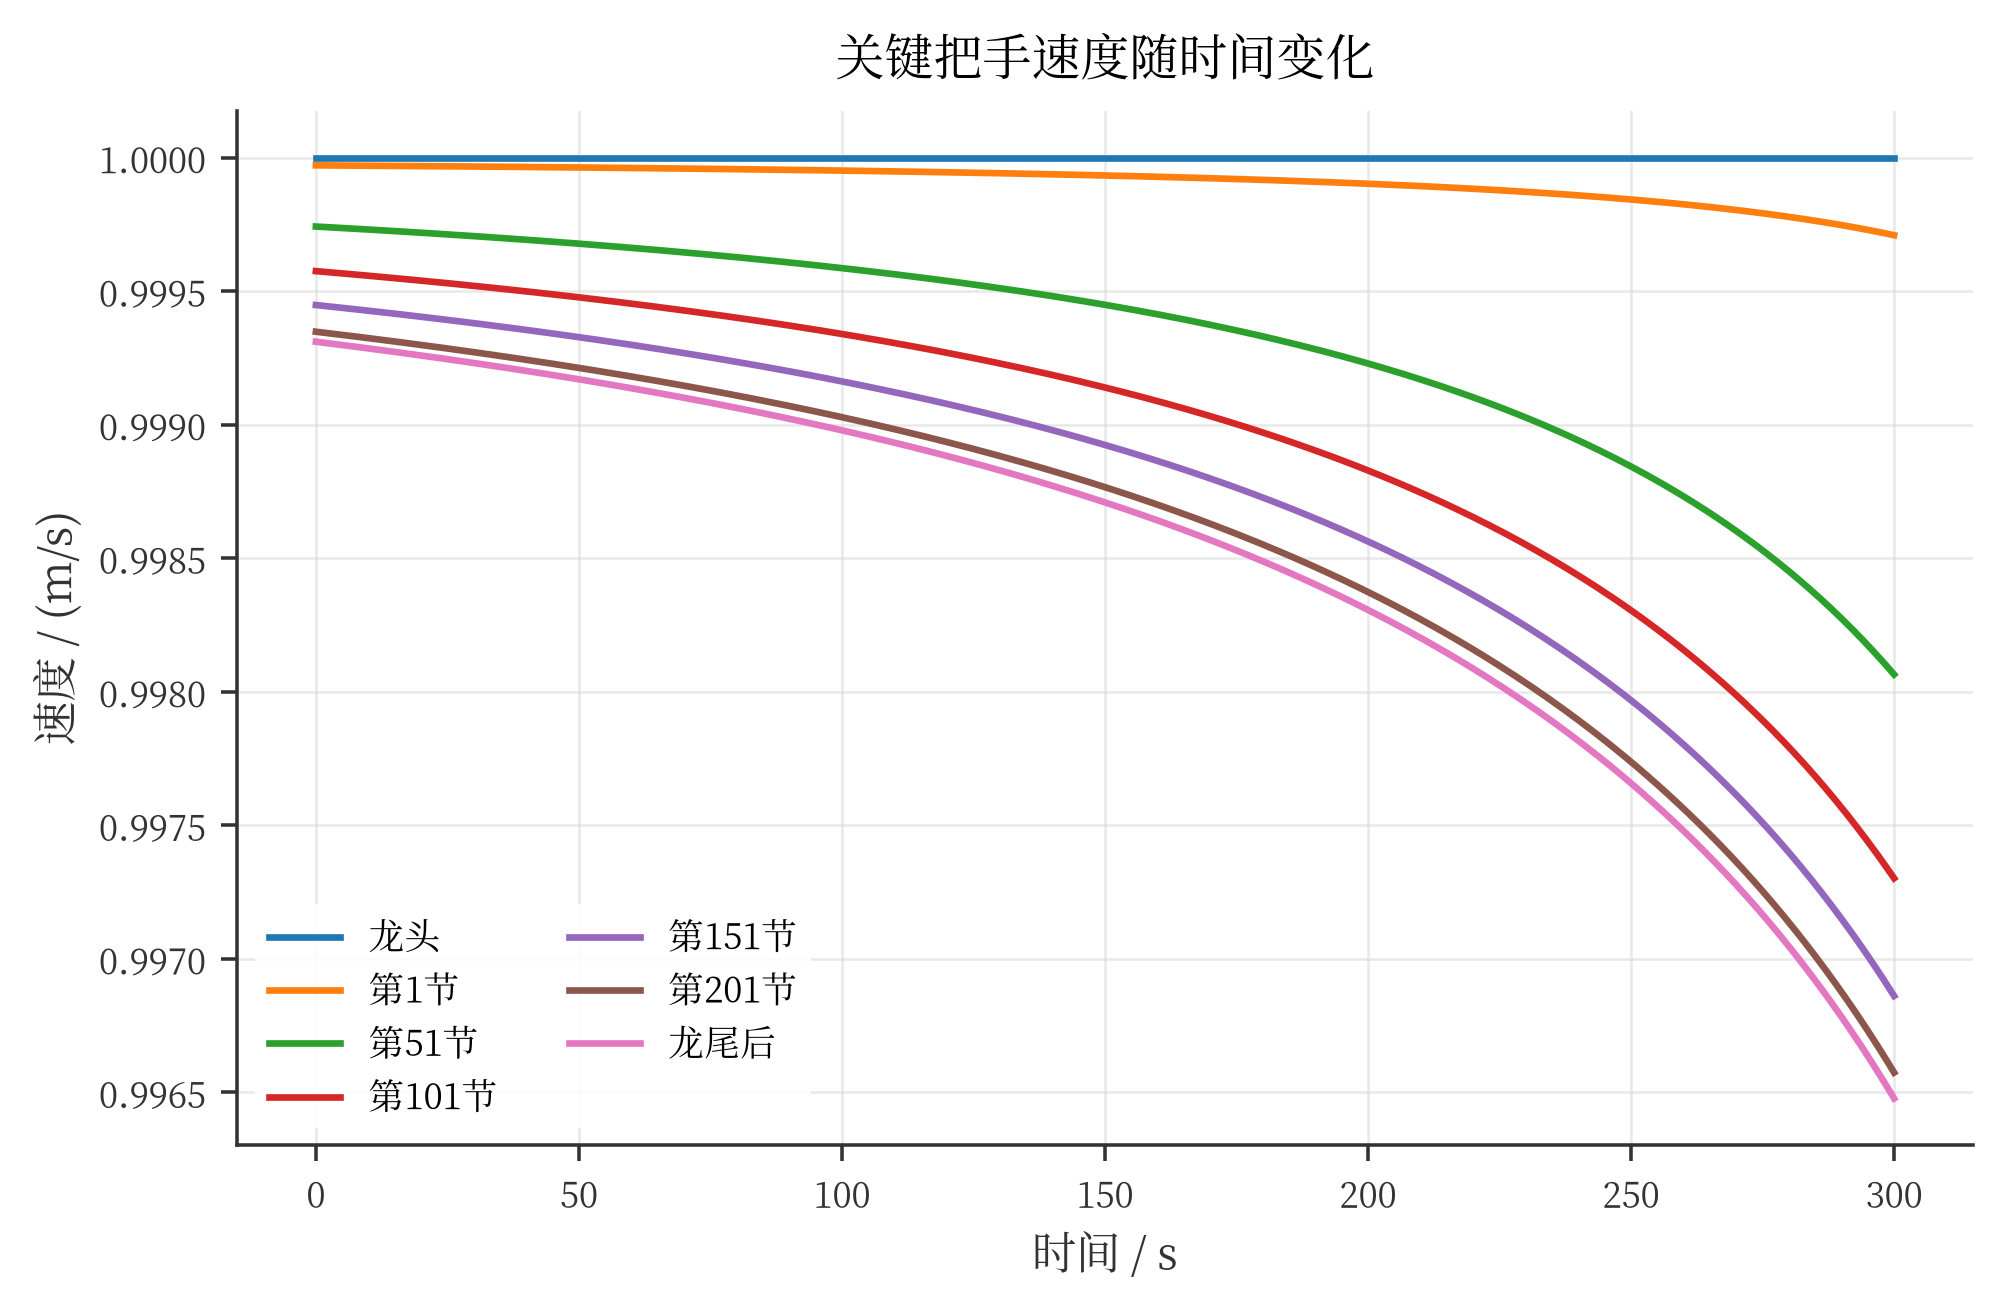
\includegraphics[width=0.88\textwidth]{figures/python/q1_key_handle_speed_time.png}
\caption{关键把手速度随时间变化}
\label{fig:q1-key-speed-time}
\end{figure}

因此，问题一的等距螺线弧长模型既满足题目对位置和速度输出的要求，也为后续碰撞判定、最小螺距搜索和调头路径建模提供了统一的几何基础。
